\documentclass[12pt]{report}

%\usepackage[utf8]{inputenc} % Codificación de entrada
\usepackage[spanish]{babel} % Packete de palabras clave en español
\renewcommand{\spanishlisttablename}{Índice de tablas} % Redefinir la traduccion de listoftables
\renewcommand{\spanishtablename}{Table} % Redefinir la traduccion de table

\usepackage[a4paper, width=150mm, top=25mm, bottom=25mm]{geometry} % Definir tamaño de hoja y margenes

\usepackage{graphicx} % Paquete para usar imagenes
\graphicspath{ {images/} } % Definir el directorio de las imagenes

\usepackage{tabularx}
\usepackage{multirow}

\usepackage{caption} % Paquete para subfiguras
\usepackage{subcaption} % Paquete para subfiguras

\usepackage{fancyhdr} % Paquete de cabeceras
\pagestyle{fancy} % Activar el estilo fancy headers 
\fancyhead{} % Iniciar la configuracion de cabecera en blanco
\fancyhead[L]{Capítulo \thechapter} % Mostrar capitulo en las esquinas superior izquierda
\renewcommand{\headrulewidth}{0.4pt} % Configurar grosor de linea de cabecera

\usepackage[style=apa]{biblatex} % Paquete para bibliografias
\addbibresource{references.bib} % Definir el archivo repositorio de bibliografias


\begin{document}

  \begin{titlepage}
  \begin{center}

    \vspace*{0.5cm}
    \Huge 
    \textbf{Diseño de sistemma fotovoltáico para el comercio Huascarán en el distrito de Yanama en Ancash}

    \vspace{0.5cm}
    \LARGE
    Autor:

    \textbf{Diego Roca}
    \vspace{1cm}

    Perfil de Tesis presentada para la obtención del\\
    título de Ingeniería Electrónica

    \vspace{1cm}
    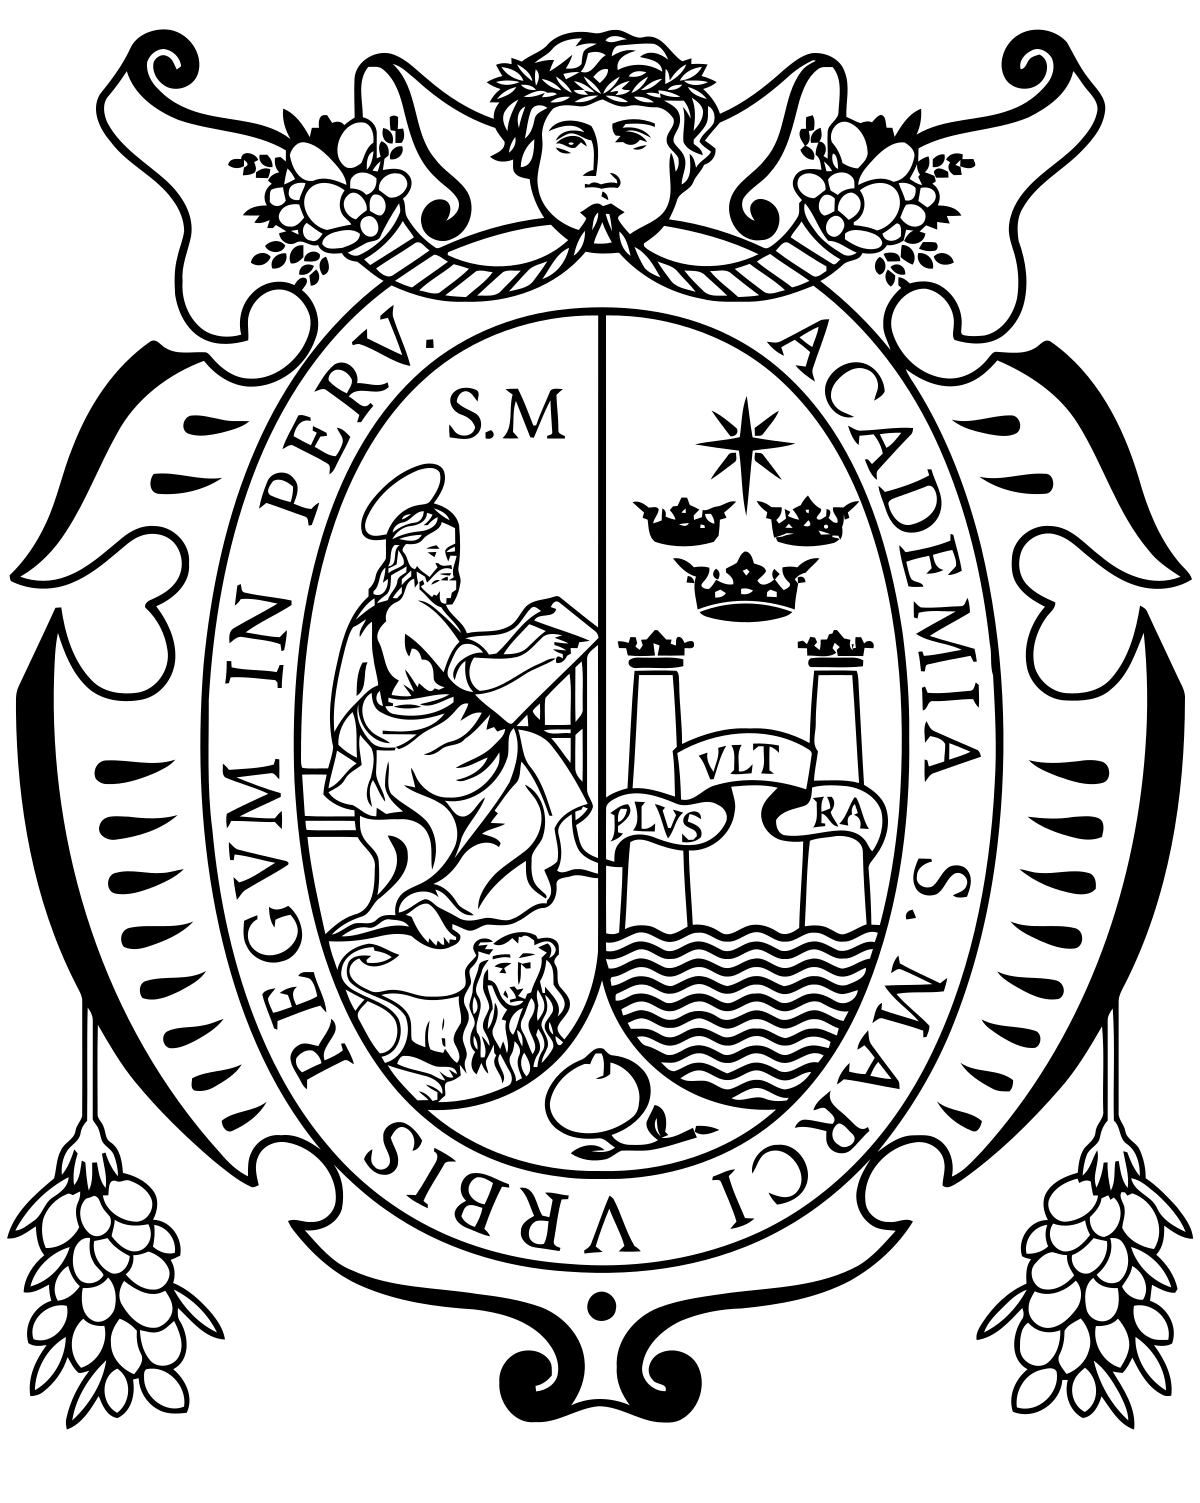
\includegraphics[width=0.5\textwidth]{universidad}

    \vfill

    \Large
    Universidad Nacional Mayor de San Marcos\\
    Perú, febrero 2025

  \end{center}
\end{titlepage}



  %\thispagestyle{plain}

\begin{center}
  \large
  \textbf{Resumen}
\end{center}

En la presente tesis se busca diseñar un guante que trackea el movimiento de las manos y reconocer los gestos que realizamos con el objetivo de poder traducir los movimiento y gestos a palabras en texto para asi tener la capacidad de traducir lenguaje de señas a texto o voz. Esto ayudaría a las personas con discapacidad auditiva a comunicarse de manera más efectiva con personas que no entienden el lenguaje de signos. Para ello se hará uso de una pequeña red neuronal que se ejecutará dentro de un pequeño microcontrolador que realizará la inferencia de la sucesión de signos y gestos que realiza la persona. En esta tesis se encontará el desarrollo completo de esta aplicación desde el diseño del hardware para el sensado, la recolección de datos, el entrenamiento de la red neuronal de clasificación y la programación del microcontrolador para ejecurar el modelo. Terminando así con un sistema embebido portátil capaz de traducir de Lenguaje de Signos Español al idioma Español hablado.
\\
\\
\textbf{Palabras clave:} inferencia, embebido, periferico, microcontrolador, entrenamiento, etiqueta, capa neuronal densa, sobreentrenamiento.

\newpage
\thispagestyle{plain}
\begin{center}
  \large
  \textbf{Abstract}
\end{center}

In this thesis, the aim is to design a glove that tracks hand movements and recognizes gestures, with the objective of translating these movements and gestures into words in text form. This capability would enable the translation of sign language into text or voice, thus helping hearing-impaired individuals to communicate more effectively with people who do not understand sign language. To achieve this, a small neural network will be employed, running on a microcontroller, to perform inference on the sequence of signs and gestures made by the user. This thesis will cover the complete development of this application, including the hardware design for sensing, data collection, training the classification neural network, and programming the microcontroller to execute the model. The result will be a portable embedded system capable of translating Spanish Sign Language into spoken Spanish.
\\
\\
\textbf{Keywords:} inference, embedded, edge device, microcontroller, training, label, fully connected layers, overfitting.


  \tableofcontents
  %\listoffigures
  %\listoftables

  %\chapter*{Introducción}
  %\addcontentsline{toc}{chapter}{Introducción}
  %Hoy en día en los dispositivos que usamos comunmente tales como las computadoras, smartphones o consolas de videojuegos interactuamos con ellos mediante periféricos tales como el teclado o el ratón. Estos a pesar de estar totalmente estandarizados tienen tambien sus limitaciones en muchas aplicaciones que requieren una interacción mas natural con las manos tales como la realidad virtual o los softwares de diseño 3D. En un dispositivo que pueda cumplir la tarea de \textit{trackear} los movimientos de nuestras manos tambien se presenta el reto de que la consola con la que estemos interactuando interprete correctamente las acciones o gestos que queremos realizar y no solo el movimiento en sí. 

Aunque para nosotros reconocer tales gestos es una tarea sumamente sencilla y para la que nuestro cerebro está entrenado, para las computadoras no lo es tanto ya que nuestros movimientos no son perfectos y por tanto cada gesto aunque sea el mismo siempre dará mediciones distintas a los sensores. Por ello en este trabajo de investigación se usará el potencial del TinyML para el reconocimiento de estos gestos. El TinyML es una rama de la inteligencia artificial cuyo desarrollo está siendo muy relevante en la acualidad y que busca entrenar modelos lo suficientemente capaces y que a la vez puedan ejecutarse en procesadores de muy bajos recursos como lo son los microcontroladores.

Esta capacidad de reconocer gestos de las manos mediante un traqueo simple puede dar lugar a plicaciones tales como: Tracking de destreza y movilidad en terapias de rehabilidación médica, como input a una computadora para usarse como periferico en programas que requieran control de un entorno 3D como videojuegos y la traduccion de lenguaje de señas a texto. Esta última será la aplicación usada como demostración del uso que puede tener el diseño del sistema de reconocimiento de gestos presentado en este trabajo de tesis.


  \chapter{Planteamiento del Problema}
  En zonas alejadas con infraestructura eléctrica limitada, los cortes frecuentes de electricidad afectan directamente el desempeño y la sostenibilidad de las actividades comerciales. Este problema no solo interrumpe las operaciones diarias, sino que también genera pérdidas económicas y reduce la calidad de los servicios ofrecidos. La dependencia de fuentes de energía no renovables, como los generadores a base de combustible, implica costos elevados y contribuye al impacto ambiental negativo, lo que resalta la necesidad de buscar alternativas más eficientes y sostenibles.
\\
\\
El diseño de un sistema fotovoltaico surge como una solución viable y adaptada a las condiciones específicas de estas regiones. Este tipo de sistema aprovecha la energía solar, una fuente abundante y renovable, para suplir la demanda energética de los comercios y garantizar la continuidad de las operaciones. Sin embargo, para que este enfoque sea efectivo, es necesario un diseño que considere las particularidades del entorno, como el nivel de irradiación solar, los patrones de consumo eléctrico del comercio, y la viabilidad económica a largo plazo. Este trabajo se enfoca en abordar estos desafíos mediante la implementación de un sistema fotovoltaico optimizado para garantizar la autosuficiencia energética en condiciones adversas.


\section{Problema Principal}
¿Cómo diseñar un sistema fotovoltaico que permita garantizar la continuidad del suministro eléctrico en el comercio Huascarán y reducir la dependencia de fuentes no renovables?

\section{Problemas Específicos}
\begin{itemize}
  \item ¿Cómo dimensionar el generador fotovoltaico para satisfacer las necesidades energéticas del comercio?
  \item ¿Cómo implementar un sistema de almacenamiento de energía que permita suplir la demanda eléctrica durante los cortes de electricidad o en horas de baja generación solar?
  \item ¿Cómo evaluar la viabilidad económica del sistema fotovoltaico, incluyendo costos de instalación, mantenimiento y el retorno de inversión esperado?
\end{itemize}



  \chapter{Justificación}
  Ante la problemática de los cortes frecuentes de energía eléctrica en el distrito de Yanama, el diseño e implementación de un sistema fotovoltaico aislado se justifica como una solución técnica y sostenible. Este sistema garantizará una fuente alternativa de alimentación eléctrica, evitando los paros operativos y asegurando la continuidad de las comunicaciones. De esta manera, se busca no solo mitigar las pérdidas económicas, sino también fortalecer la estabilidad operativa del comercio frente a las limitaciones del suministro energético convencional.
\\
\\
Además de solucionar los problemas los problemas mencionados, el sistema fotovoltaico aislado presenta la posibilidad de sustituir parcialmente el suministro eléctrico convencional durante ciertas jornadas de trabajo. Esto permitiría reducir significativamente los costos asociados al consumo de energía a largo plazo.

\section{Justificación Metodológica}
La metodología empleada en este trabajo se basa en análisis técnico, evaluación de la demanda energética y la selección de componentes óptimos, permitiendo desarrollar una solución eficiente, confiable y adaptada al contexto del comercio.

\section{Justificación Teórica}
El diseño de sistemas fotovoltaicos aislados se fundamenta en principios de conversión de energía solar, eficiencia energética y sostenibilidad. Este trabajo se basa en teorías de generación distribuida y almacenamiento energético, y busca contribuir al conocimiento práctico sobre cómo implementar soluciones autónomas en áreas donde el suministro eléctrico es inestable.

\section{Justificación Práctica}
El desarrollo del sistema fotovoltaico aislado para el comercio Huascarán tendrá un impacto directo en la continuidad de sus operaciones, reduciendo pérdidas económicas por cortes eléctricos. Asimismo, permitirá una reducción de costos operativos mediante el aprovechamiento de energía solar durante jornadas laborales específicas. 


  \chapter{Marco Teórico}
  El marco tenorico necesario para abordar la investicación se basa en los siguientes conceptos

\begin{itemize}

  \item \textbf{Energía y Radiación Solar}

  La energía solar es una fuente renovable obtenida directamente del Sol mediante la captación de su radiación electromagnética. Esta radiación, compuesta por radiación directa, difusa y global, varía según factores como la latitud, la altitud y las condiciones climáticas de una región. En el caso del distrito donde opera el comercio Huascarán, la alta disponibilidad de radiación solar lo convierte en un lugar ideal para la implementación de sistemas fotovoltaicos, aprovechando al máximo esta fuente energética limpia y abundante.


  \item \textbf{Sistemas Fotovoltáicos Aislados}

  Los sistemas fotovoltaicos aislados son soluciones energéticas diseñadas para operar de manera independiente a la red eléctrica convencional. En este caso el sistema actuará como una fuente alternativa cuando la red presente algun corte. Estos sistemas utilizan paneles solares para captar energía, que luego es almacenada en baterías para garantizar un suministro constante. Su implementación es especialmente útil en áreas donde el acceso a la red es inestable, como en el caso del comercio Huascarán, proporcionando una fuente confiable y autónoma de energía.


  \item \textbf{Almacenamiento de energía}

  El almacenamiento de energía es una parte esencial de los sistemas fotovoltáicos aislados, ya que permite acumular la energía generada durante el día para su uso en horas nocturnas o en momentos de baja radiación solar. Actualmente la solución más extendida y más práctica son las baterías quimicas, como las de plomo-ácido o litio-ion, debido a su capacidad de almacenar grandes cantidades de energía y su vida útil prolongada. En este proyecto, el correcto dimensionamiento y selección de las baterías garantiza un suministro continuo para las operaciones del comercio Huascarán.


  \item \textbf{Dimensionamiento}

  El dimensionamiento de un sistema fotovoltáico aislado implica calcular la capacidad y cantidad de componentes necesarios para satisfacer las necesidades energéticas específicas del usuario. Este proceso incluye el análisis de la demanda energética diaria, la estimación de la radiación solar disponible y la consideración de factores como pérdidas y eficiencia del sistema. Para el comercio Huascarán, el dimensionamiento asegura que el sistema diseñado sea capaz de soportar las cargas críticas durante las operaciones, incluso en condiciones adversas.


  \item \textbf{Cultura de mantenimiento de sistemas fotovoltáicos}

  La cultura de mantenimiento en sistemas fotovoltaicos se refiere a la adopción de prácticas regulares, preventivas y correctivas para asegurar el óptimo desempeño del sistema a lo largo de su vida útil. Este concepto no solo implica realizar intervenciones técnicas específicas, sino también fomentar una mentalidad proactiva en los poseedores del sistema, quienes deben entender la importancia de estas actividades para evitar fallos y maximizar la inversión realizada.

\end{itemize}


  \chapter{Antecedentes}
  \section{Internacionales}

\begin{itemize}
  
  \item \textbf{Sistema Solar Fotovoltaico Aislado Para el Suministro de Energía Eléctrica a una vivienda Rural \parencite{Mestre}}

El proyecto plantea como solución el diseño e implementación de un sistema solar fotovoltaico aislado para abastecer de energía eléctrica a una vivienda rural en la zona de Patillal, Cesar, Colombia, caracterizada por su déficit energético y difícil acceso a la red eléctrica convencional. Se evalúan las necesidades energéticas de una vivienda típica, se seleccionan los componentes necesarios del sistema (paneles solares, regulador, inversor, baterías), y se realizan cálculos para dimensionar su capacidad. Concluye que este sistema es económicamente viable al recuperar la inversión en un tiempo razonable.

  \item \textbf{Diseño de un Sistema de Generación Fotovoltaico Residencial Autónomo para el Consumo Nivel 1 \parencite{Dominguez}}

Este trabajo describe el diseño de un sistema de generación fotovoltaico residencial autónomo, orientado a suplir las necesidades de consumo eléctrico de viviendas en áreas rurales de Ecuador, particularmente en San Juan de Ilumán. A partir de la estimación de demanda energética y condiciones locales de radiación solar, se dimensionaron los componentes necesarios: paneles solares, baterías, inversores, reguladores y conductores. El proyecto concluye que, debido a la alta radiación solar constante en Ecuador, esta tecnología es sostenible y eficaz, mejorando la calidad de vida y promoviendo el uso de energía limpia y renovable, a la vez que respalda el cuidado ambiental.

  \item \textbf{Diseño de un sistema aislado para el uso en casas flotantes en la ciudad de Babahoyo \parencite{Puco}}

El documento aborda el diseño de un sistema fotovoltaico aislado para abastecer de energía eléctrica a casas flotantes ubicadas en Babahoyo, Ecuador, en áreas de difícil acceso a la red eléctrica. Con un enfoque experimental, descriptivo y documental, el estudio evalúa la irradiancia local y los componentes requeridos, como paneles solares, baterías, inversores y controladores de carga. Se concluye que esta alternativa es viable, ya que mejora la calidad de vida de los residentes al proporcionar energía renovable y reduce la dependencia de combustibles fósiles, promoviendo la sostenibilidad ambiental.

\end{itemize}


\section{Nacionales}

\begin{itemize}
    
    \item \textbf{Análisis Comparativo de Rendimientos Entre un Sistema Fotovoltaico con Seguidor Solar de Doble Eje y un Distema Fotovoltaico de Montura Fija \parencite{Laureano}}


    \item \textbf{Análisis Costo Beneficio Del Sistema Fotovoltáico Monofásico Conectado a la Red \parencite{Guevara}}


    \item \textbf{Diseño de un Sistema Fotovoltaico con Seguidor Solar para Sistema de Telecomunicación de las Subestaciones Sector Norte \parencite{Correa}}


\end{itemize}


  \chapter{Objetivos}
  \section{Objetivo Principal}
Diseñar un sistema fotovoltaico que permita garantizar la continuidad del suministro eléctrico en el comercio Huascarán y reducir la dependencia de fuentes no renovables

\section{Objetivos espcíficos}
\begin{itemize}
  \item Dimensionar el generador fotovoltaico para satisfacer las necesidades energéticas del comercio
  \item Implementar un sistema de almacenamiento de energía que permita suplir la demanda eléctrica durante los cortes de electricidad o en horas de baja generación solar
  \item Evaluar la viabilidad económica del sistema fotovoltáico, incluyendo costos de instalación, mantenimiento y el retorno de inversion esperado
\end{itemize}


  \chapter{Hipótesis}
  \section{Hipótesis Principal}
El sistema fotovoltaico permite garantizar la continuidad del suministro eléctrico en el comercio Huascarán y reduce la dependencia de fuentes no renovables

\section{Hipótesis Específicas}
\begin{itemize}
  \item El generador fotovoltaico satisface las necesidades energéticas del comercio
  \item El sistema de almacenamiento de energía permite suplir la demanda eléctrica durante los cortes de electricidad o en horas de baja generación solar
  \item Es viable económicamente el sistema fotovoltaico, incluyendo costos de instalación, mantenimiento y el retorno de inversión esperado
\end{itemize}


  \chapter{Variables}
  \section{Variables independientes}

\begin{center}
\begin{tabularx}{\textwidth} { 
  | >{\centering\arraybackslash}X 
  | >{\centering\arraybackslash}X 
  | >{\centering\arraybackslash}X
  | >{\centering\arraybackslash}X
  | >{\centering\arraybackslash}X | } \hline

  VARIABLES & DEF. CONCEPTUAL & DEF. OPERACIONAL & DIMENSIO-NES & INDICADO-RES \\ \hline

  \vspace{1.2cm} \multirow{3}{*}{\begin{tabular}[c]{@{}l@{}}Reconocimien-\\ to de gestos \\ del LSP\end{tabular}} & 
  \vspace{1.2cm} \multirow{3}{*}{\begin{tabular}[c]{@{}l@{}}Rendimiento\\ del sistema \\ reconociendo \\ gestos\end{tabular}} & 
  \vspace{1.2cm} \multirow{3}{*}{\begin{tabular}[c]{@{}l@{}}Será medido a\\ traves de \\ los resultados \\ arrojados por \\ el sistema\end{tabular}} & 
  \vspace{1.3cm} \multirow{2}{*}{\begin{tabular}[c]{@{}l@{}}Precisión\end{tabular}} & 
  \vspace{0.2cm} Tasa de aciertos\\ 
  \cline{5-5}

   &  &  &  & \vfill Matriz de confusión \vfill \\ \cline{4-5}

   &  &  & \vspace{0.3cm} Eficiencia \vfill & \vfill Tiempo de respuesta \vfill \\ \hline

\end{tabularx}
\end{center}

\section{Variables dependientes}

\begin{center}
\begin{tabularx}{\textwidth} { 
  | >{\centering\arraybackslash}X 
  | >{\centering\arraybackslash}X 
  | >{\centering\arraybackslash}X
  | >{\centering\arraybackslash}X
  | >{\centering\arraybackslash}X | } 
  \hline

  VARIABLES & DEF. CONCEPTUAL & DEF. OPERACIONAL & DIMENSIO-NES & INDICADO-RES \\ \hline

  \vspace{0.4cm} \multirow{3}{*}{\begin{tabular}[c]{@{}l@{}}Modelo entre- \\ nado y hard- \\ ware\end{tabular}} & 
  \vspace{0.4cm} \multirow{3}{*}{\begin{tabular}[c]{@{}l@{}}Implementa-\\ ción del mode- \\ lo y hardware\end{tabular}} & 
  \vspace{0.4cm} \multirow{3}{*}{\begin{tabular}[c]{@{}l@{}}Será medido a\\ traves de ...\end{tabular}} & 
  \vfill Modelo \vfill & 
  \vfill Entrenamiento \vfill \\ 
  \cline{4-5}

   &  &  & \vspace{0.35cm} Hardware \vfill & \vfill Implementa-ción \vfill \\ \hline

\end{tabularx}
\end{center}

  
  \chapter{Materiales y Metodos}
  \section{Equipos, Materiales y Servicios}

Para el desarrollo de esta investigación se empleará el siguiente equipo:

\begin{itemize}
  \item Laptop con Procesador Core i3 con 8GB de RAM
  \item Pinza Amperimétrica
  \item Software Matlab
  \item Software PVsyst
  \item Software Helioscope
\end{itemize}

\section{Métodos}
\subsection{Diseño y alcanze de la investigación}

La presente investigación será de tipo aplicada debido a que este proyecto tiene como objetivo desarrollar una solución concreta (el sistema fotovoltaico) para un problema real (los cortes eléctricos que afectan al comercio Huascarán).
\\
\\
Se plantea además un enfoque cuantitativo ya que el diseño del sistema requiere cálculos precisos, como el dimensionamiento de paneles, baterías e inversores, así como la estimación de costos y la evaluación del desempeño energético.
\\
\\
El alcance de esta investigación es describir las condiciones actuales del comercio (problemas energéticos) y las características del sistema propuesto, detallando componentes, funcionamiento y beneficios.
\\
\\
El proyecto no incluye pruebas ni cambios en el sistema eléctrico del comercio Huascarán. El análisis se realiza desde una perspectiva teórica por lo que es un trabajo no experimental.

\subsection{Población y Muestra}

Debido a la naturaleza de la investigación, no se define una población ni una muestra en el sentido convencional. Este trabajo se enfoca exclusivamente en el diseño de un sistema fotovoltaico aislado para el comercio Huascarán, el cual representa un caso particular con características específicas. Si bien los resultados pueden servir como referencia para situaciones similares, el estudio no busca generalizar a un conjunto mayor de establecimientos.

\subsection{Técnicas o métodos a aplicar}

\begin{itemize}

  \item Reecolección de Inromacion documental: Se recopilará y analizará información de fuentes como libros, articulos, normatibas, manuales técncos y bases de datos.
  
  \item Análisis de datos técnicos: Se evaluará los datos específicos, como el consumo energético del comercio, los niveles de radiación solar en la región y las especificaciones técnicas de los equipos disponibles.

  \item Calculos de dimensionamiento: basado en fórmulas y estándares técnicos para determinar la capacidad y cantidad de paneles solares, baterías e inversores necesarios.

  \item Simulacion Energética: Uso de herramientas o software para simular el comportamiento del sistema bajo diferentes condiciones.

  \item Análisis de Viabilidad Técnica y Económica: Evaluar los costos de instalación y operación y mantenimiento, comparándolos con los beneficios energéticos y económicos del sistema para determinar si el sistema es rentable para el comercio Huascarán

  \item Revisión Normativa: Estudio de normativas y estándares nacionales o internacionales relacionados con sistemas fotovoltaicos aislados para asegurar que el diseño cumpla con las regulaciones vigentes, garantizando seguridad y funcionalidad.

\end{itemize}


  \chapter{Cronograma de actividades}
  El cronograma par el desarrollo de la investigación se presenta a continuación:

\begin{center}
\begin{table}[h]
\caption{Cronograma de la investigación}
\begin{tabularx}{\textwidth} { 
  | >{\raggedright\arraybackslash}X
  | >{\centering\arraybackslash}p{3cm} | } \hline

  \textbf{ETAPA DE LA INVESTIGACIÓN}          & \textbf{DURACIÓN (DIAS)} \\ \hline
  Desarrollo del marco teórico                & 2                        \\ \hline
  Planteamiento metodológico                  & 2                        \\ \hline
  Ejecución de la investigación 
  (sistematización de muestras, entrenamienti 
  y validación)                               & 10                       \\ \hline
  Obtención y análisis de indicadores         & 4                        \\ \hline
  Implementación del prototipo                & 2                        \\ \hline
  Análisis de resultados                      & 5                        \\ \hline 
  Integración de la versión final de la Tesis & 4                        \\ \hline 
  DURACIÓN TOTAL                              & 30                       \\ \hline 
  
\end{tabularx}
\end{table}
\end{center}


  \chapter{Metas}
  Las metas de la investigación se definirán en función a los procesos definidos
en la metodología, los cuales se presentan a continuación:

\begin{center}
\begin{table}[h]
\caption{Metas de la investigación}
\begin{tabularx}{\textwidth} { 
  | >{\raggedright\arraybackslash}X
  | >{\raggedright\arraybackslash}p{6cm} | } \hline

  \textbf{ETAPA DE LA INVESTIGACIÓN}          & \textbf{DURACIÓN (DIAS)} \\ \hline
  Desarrollo del marco teórico                & Marco teórico, antecedentes y afines desarrollados.                        \\ \hline
  Planteamiento metodológico                  & Metodología de la investigación, definición de variables e indicadores y su operacionalización                        \\ \hline
  Ejecución de la investigación 
  (sistematización de muestras, entrenamienti 
  y validación)                               & Modelos entrenados integrados para la detección y reconocimiento de las placas de rodaje                       \\ \hline
  Obtención y análisis de indicadores         & Indicadores calculados a partir de los modelos entrenados para elección del mejor                        \\ \hline
  Implementación del prototipo                & Prototipo para el reconocimiento de placas empleando la tarjeta Raspberry Pi 4                        \\ \hline
  Análisis de resultados                      & Análisis de resultados del prototipo                        \\ \hline 
  Integración de la versión final de la Tesis & Documento de Tesis finalizado                        \\ \hline 
  DURACIÓN TOTAL                              & 30                       \\ \hline 
  
\end{tabularx}
\end{table}
\end{center}


  \chapter{Presupuesto}
  Se estima un presupuesto de 1500 soles cuyos itmes se detallan en la siguiente tabla

\begin{center}
\begin{table}[h]
\caption{Presupuesto de la investigación}
\begin{tabularx}{\textwidth} { 
  | >{\raggedright\arraybackslash}X
  | >{\centering\arraybackslash}p{3cm} | } \hline

  \textbf{ITEM}             & \textbf{COSTO}      \\ \hline
  Paneles Solares           & 120                 \\ \hline
  Baterías                  & 80                  \\ \hline
  Sistema de Regulación     & 30                  \\ \hline
  Sistema de Adaptacíón     & 700                 \\ \hline
  Cableado                  & 100                 \\ \hline
  Accesoriosnn              & 60                  \\ \hline 
  TOTAL                     & 1090                \\ \hline 
  
\end{tabularx}
\end{table}
\end{center}


  \printbibliography

\end{document}
